As previously described, the generalized Gauss-Newton matrix arises from the partial linearization of a composite function.
In our case, we will linearize the neural network predictions $f_n \to f_n^{\text{lin}} = \lin_{\vtheta_0}(f_n)$, then form the partially-linearized per-sample losses $\tilde{\ell}_n = c_n \circ f_n^{\text{lin}}$ which themselves give rise to the partially linearized empirical risk $\tilde{\gL}_{\sD}(\vtheta) = R \sum_{n=1}^{N} \tilde{\ell}_n(\vtheta)$.
We then define the vec GGN matrix of $\gL_{\sD}(\vtheta)$ as the Hessian of the partially-linearized empirical risk where the linearization is anchored at the evaluation point of the GGN, just like in \Cref{sec:partial_linearization},
\begin{align*}
  \ggn^{\vec}_{\vtheta} \gL_{\sD}(\vtheta)
  &=
  \left.\hess_{\vtheta}^{\vec} \tilde{\gL}_{\sD}(\vtheta)\right|_{\vtheta_0 = \vtheta} \in \sR^{D \times D}
    \\
  &=
    R \sum_{n=1}^N
    \left.\hess_{\vtheta}^{\vec} \tilde{\ell}_n(\vtheta)\right|_{\vtheta_0 = \vtheta},
\end{align*}
where $\vec$ is one of the flattening operations.
We can also express the GGN through Jacobians,
\begin{align*}
  &\ggn^{\vec}_{\vtheta} \gL_{\sD}(\vtheta)
  \\
  &=
  R \sum_{n=1}^N
  [\jac_{\vtheta}^{\vec} f_n]^{\top}
  [\hess^{\vec}_{f_n} \underbrace{c_n(f_n)}_{\ell_n}]
  [\jac_{\vtheta}^{\vec} f_n].
\end{align*}

\switchcolumn[1]
\begin{figure}
  \centering
  \begin{minipage}[t]{0.495\linewidth}
    \centering
    $\cvec$\vspace{1ex}
    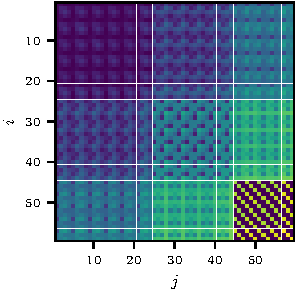
\includegraphics[width=\linewidth]{../kfs/plots/synthetic_cvec_ggn.pdf}
  \end{minipage}
  \hfill
  \begin{minipage}[t]{0.495\linewidth}
    \centering
    $\rvec$\vspace{1ex}
    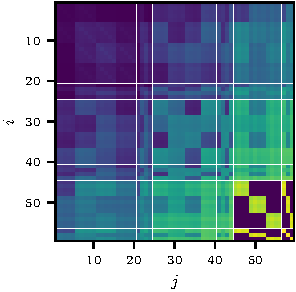
\includegraphics[width=\linewidth]{../kfs/plots/synthetic_rvec_ggn.pdf}
  \end{minipage}
  \\
  \begin{minipage}[t]{0.495\linewidth}
    \centering
    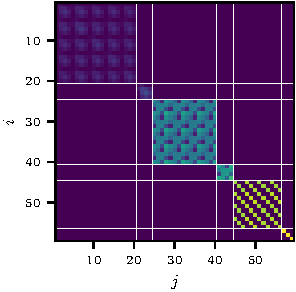
\includegraphics[width=\linewidth]{../kfs/plots/synthetic_cvec_ggn_bda.pdf}
  \end{minipage}
  \hfill
  \begin{minipage}[t]{0.495\linewidth}
    \centering
    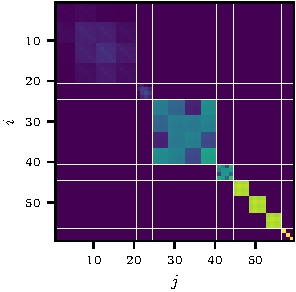
\includegraphics[width=\linewidth]{../kfs/plots/synthetic_rvec_ggn_bda.pdf}
  \end{minipage}
  \caption{Visualization of the GGN and its block-diagonal approximation using different flattening schemes.
    The GGN blocks are visually highlighted with white lines.
    Left column uses $\cvec$-flattening, right column uses $\rvec$-flattening.
    The GGN was evaluated on synthetic data ($N=100$) using an MLP with three fully-connected layers and ReLU activations (5-4-4-3, our notation considers applying the weight matrix and adding the bias as two layers, hence $L=6$) and square loss.
  }
\end{figure}

\switchcolumn[0]
Just like the Hessian, the GGN has a block structure. With the abbreviations
$\ggn_{k,l}^{\vec}\gL \coloneq \ggn^{\vec}_{\vtheta^{(k)}, \vtheta^{(l)}} \gL_{\sD}(\vtheta) = \hess^{\vec}_{\vtheta^{(k)}, \vtheta^{(l)}} \tilde{\gL}_{\sD}(\vtheta) = R \sum_{n=1}^N [\jac_{\vtheta^{(k)}}^{\vec} f_n]^{\top} [\hess^{\vec}_{f_n} c_n(f_n)] [\jac_{\vtheta^{(l)}}^{\vec} f_n]$ and $\ggn_{k}^{\vec}\gL \coloneq \ggn^{\vec}_{\vtheta^{(k)}} \gL_{\sD}(\vtheta)$, we can write the GGN as
\begin{align*}
  \ggn_{\vtheta}^{\vec} \gL
  =
  \begin{pmatrix}
    \ggn_1^{\vec} \gL
    &
      \ggn_{1, 2}^{\vec} \gL
    &
      \cdots
    &
      \ggn_{1, L}^{\vec} \gL
    \\
    \ggn_{2, 1}^{\vec} \gL
    &
      \ggn_2^{\vec} \gL
    &
      \cdots
    &
      \ggn_{2, L}^{\vec} \gL
    \\
    \vdots & \cdots & \ddots & \vdots
    \\
    \ggn_{L, 1}^{\vec} \gL
    &
      \ggn_{L, 2}^{\vec} \gL
    &
      \cdots
    &
      \ggn_L^{\vec} \gL
  \end{pmatrix}\,.
\end{align*}
In the following, we will only consider the block diagonal approximation of this matrix,
\begin{align*}
  \tilde{\ggn}_{\vtheta}^{\vec} \gL
  =
  \begin{pmatrix}
    \ggn_1^{\vec} \gL & \vzero & \cdots & \vzero
    \\
    \vzero & \ggn_2^{\vec} \gL & \ddots & \vdots
    \\
    \vdots & \ddots & \ddots & \vzero
    \\
    \vzero & \cdots & \vzero & \ggn_L^{\vec} \gL
  \end{pmatrix}\,,
\end{align*}
\ie, individual blocks $\{ \ggn_{\vtheta^{(k)}}^{\vec} \gL_{\sD}(\vtheta)\}_{k=1}^L$.

\paragraph{The GGN as a self-outer product}
Let us look at the GGN contributed by a single datum and suppress the index $_n$ for now, as well as the reduction factor $R$.
This contribution is
\begin{align*}
  \underbrace{[\jac_{\vtheta}^{\vec} f]^{\top}}_{\dim(\Theta) \times \dim(\gF)}
  \underbrace{[\hess^{\vec}_{f} c(f)]}_{\dim(\gF) \times \dim(\gF)}
  \underbrace{[\jac_{\vtheta}^{\vec} f]}_{\dim(\gF) \times \dim(\Theta)}\,.
\end{align*}
We will now make this more symmetric.
Note that, by assumption, the criterion function $c$ is convex in $f$.
This means that the flattened Hessian $\hess^{\vec}_{f} c(f)$ is positive semi-definite.
Since any positive semi-definite matrix $\mA \in \sR^{C \times C}$ can be expressed as an outer product $\mA = \mB \mB^{\top}$ where $\mB \in \sR^{C \times \rank(\mA)}$, we can find a symmetric factorization $\mS^{\vec} \in \sR^{\dim(\gF) \times \dim(\gF)}$ of the criterion's Hessian such that $\hess^{\vec}_{f} c(f) = \mS^{\vec} {\mS^{\vec}}^{\top}$.
With that, we can then write the upper expression as
\begin{align*}
  &[\jac_{\vtheta}^{\vec} f]^{\top} \mS^{\vec} {\mS^{\vec}}^{\top} [\jac_{\vtheta}^{\vec} f]
  \\
  &=
  \underbrace{([\jac_{\vtheta}^{\vec} f]^{\top} \mS^{\vec})}_{\coloneq \mV^{\vec} \in \sR^{\dim(\Theta) \times \dim(\gF)}}
  ([\jac_{\vtheta}^{\vec} f]^{\top} \mS^{\vec})^{\top}
  \\
  &=
  \mV^{\vec} {\mV^{\vec}}^{\top}\,.
\end{align*}
I.e., we can express the flattened GGN contribution of a single datum as a self-outer product.
In the following, we will not look further into $\mV^{\vec}$; see~\cite{dangel2022vivit,papyan2019measurements} for a detailed discussion. Instead, we want to derive the factorization for the Hessian of the square and cross-entropy losses, which will become useful in later chapters.
\begin{example}[Symmetric factorization of the Hessian of square loss]\label{ex:mseloss_hessian_factorization}
  Consider the square loss $c$ from \Cref{ex:square_loss} and its Hessian from \Cref{ex:square_loss_hessian}.
  The Hessian's symmetric factorization is simply
  \begin{align*}
    \mS^{\vec} = \mI
  \end{align*}
  because $\mS^{\vec} {\mS^{\vec}}^{\top} = \mI = \hess_{f}^{\vec}c$.
\end{example}

\begin{example}[Symmetric Hessian decomposition of softmax cross-entropy loss, \Cref{hessian_factorizations}]\label{ex:crossentropyloss_hessian_factorization}
  The Hessian's symmetric factorization is \citep[\eg][]{papyan2019measurements}
  \begin{align*}
    \mS^{\vec} = \diag(\sqrt{\vp}) - \vp \sqrt{\vp}^{\top}
  \end{align*}
  where $\vp = \softmax(\vf)$ and the square root is applied element-wise.
  To see this, we can form $\mS^{\vec} {\mS^{\vec}}^{\top}$ which yields
  \begin{align*}
    \diag(\vp) - 2 \vp \vp^{\top} + \vp \sqrt{\vp}^{\top} \sqrt{\vp} \vp^{\top}
    \\
    = \diag(\vp) - \vp \vp^{\top}
  \end{align*}
  using the fact that $\vp^{\top} \vone = 1 = \sqrt{\vp}^{\top} \sqrt{\vp}$.
  This expression equals the Hessian from \Cref{ex:square_loss_hessian}.
\end{example}
Note that the Hessian factorization for both the square loss and the softmax cross-entropy loss do not depend on the label, \ie, the second argument of the criterion function.
We will make use of this property in the next section to connect the GGN with the Fisher matrix for regression and classification tasks.

%%% Local Variables:
%%% mode: latex
%%% TeX-master: "../main"
%%% End:
